\documentclass{article}
 
\usepackage[margin=1in]{geometry}
\usepackage{amsmath,amsthm,amssymb}
\usepackage{booktabs}
\usepackage{enumitem,epsfig}
\usepackage{graphicx}
\usepackage{rotating}
\usepackage{multirow}
\usepackage{float}
\usepackage{tikz}

\newcommand*\encircle[1]{%
\tikz[baseline=(C.base)]\node[draw,circle,inner sep=0.5pt](C) {#1};
}

\def\x{\mathbf{x}}
\def\y{\mathbf{y}}
\def\v{\mathbf{v}}
\def\a{\mathbf{a}}
\def\b{\mathbf{b}}
\def\ttheta{(1-\theta)}
\def\A{\mathbf{A}}
\def\F{\mathbf{F}}
\def\I{\mathbf{I}}
\def\R{\mathbb{R}}
\def\C{\mathcal{C}}
\def\L{\mathcal{L}}

 
\begin{document}
 
\title{ECE 466 Midterm 2}
\author{Name: \\PID: }
 
\maketitle
 
\begin{itemize}
    \item Don't forget to write your name.
    \item Open textbook. You can use your calculators.
    \item Read carefully and write legibly. For the problems with partial credit, show your work.
    \item For those of you who are remotely solving the exam: 
    \begin{itemize}
        \item You can solve your exam in A-4 sheets or on your tablet.
        \item You need to send a scanned pdf or image until 11:45 AM, to sofuoglu@msu.edu. Otherwise, your exam will not be accepted.
        \item Make sure your answers are legible from pdf or scanned image. 
    \end{itemize}
\end{itemize}

\begin{enumerate}
%%%%%%%%%%%%%%%%%%%%%%%%%%%%%%%%%%%%%%%%%%%%%%%%%%%%%%%%%%%%%%%%%%%%%%%%%%%%%% 1
    \item  {[35 points]}
    \begin{enumerate}
        \item {[5]} The DFT of a 5-point signal $x[n]$ is $X[k] = [\underline{5},6,1,2,9]$. A new signal is defined by $y[n]=e^{-j4\pi n/5}x[n]$. What are the DFT coefficients $Y[k]$ corresponding to $y[n]$? 
        \begin{figure}[H]
            \centering
            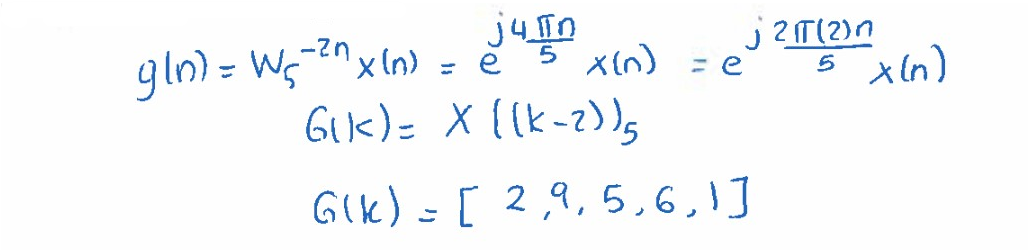
\includegraphics[width=.7\textwidth]{mt2_q1_a.png}
        \end{figure}
        \item {[5]} A signal $x[n]$ has DTFT of form $X(\omega) = \frac{1}{1-ae^{-j\omega}}$. If $Y(\omega) = \frac{e^{j\omega/2}}{1-ae^{-j\omega/2}}$, what is $y[n]$ in terms of $x[n]$?
        \begin{figure}[H]
            \centering
            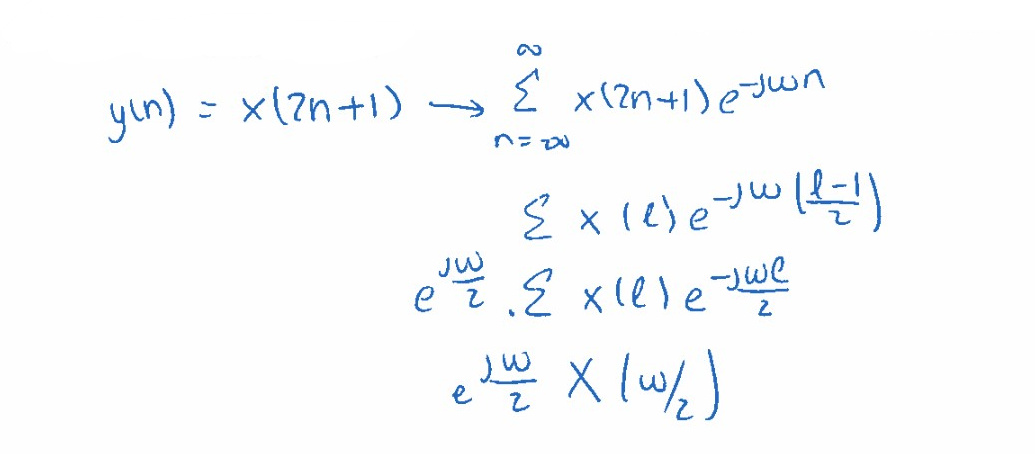
\includegraphics[width=.7\textwidth]{mt2_q1_b.png}
        \end{figure}
        \item {[5]} What is the DTFT of the signal $x[n] = \{0.5,0.5,\underline{1},0.5,0.5\}$? 
        \vspace{1in}
        \item {[5]} Using the result of part c) calculate the DTFS coefficients of the periodic signal $y[n]$, where the values over one period is given by $y[n] = \{\dots,\underline{1},0.5,0.5,0.5,0.5,\dots\}$.
        \vspace{2in}
        \item {[5]} For a given signal $x[n] = \{9,3,0,\underline{5},0,3,4\}$, what is $\int_{\pi}^\pi X(\omega) cos(2\omega) d\omega$? {\it Hint: You don't need to compute $X(\omega)$.}
        \vspace{1in}
        \item {[5]} Consider an FIR filter described by the difference equation $y[n] = x[n]-x[n-6]$. Determine it's response to $x[n] = 5 + \cos\left(\frac{2\pi}{3}n+\frac{\pi}{2}\right)$.
        \begin{figure}[H]
            \centering
            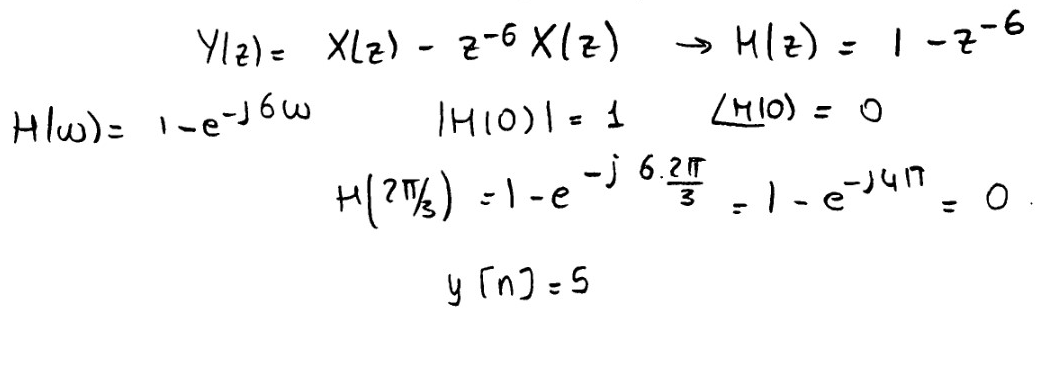
\includegraphics[width=.8\textwidth]{mt2_q1_f.png}
        \end{figure}
        \item {[5]} Let $X(z)=\frac{1+2.5z^{-1}+1.5z^{-2}}{(1+2z^{-1})\left(1+\frac{2}{5}z^{-1}-\frac{3}{5}z^{-2}\right)}$. What is the ROC, such that DTFT of this signal exists?
    \end{enumerate}

    \vspace{1in}
    \item {[30 Points]} Let $x[n]=\{\underline{1},3,2,1\}$ be the input to an LTI system with an unknown impulse response $h[n]$. The output of the system is $y[n] = {1,5,10,12,9,4,1}$.
    \begin{enumerate}
        \item {[5]} Find the length of (the non-zero part of) the impulse response $h[n]$.
        \item {[5]} What is the smallest length DFT, $N$, that is required such that $Y[k] = X[k]H[k]$.
        \item {[5]} Let $y_1[n]$ be four point circular convolution of $x[n]$ and $h[n]$, i.e. $y_1[n] = x[n] \encircle{4} h[n] $. Determine $y_1[n]$.
        \item {[7]} Find $h[n]$ using the $N$ found in part b). 
        \item {[8]} Write the difference equation corresponding to this system.
    \end{enumerate}
    \begin{figure}[H]
        \centering
        
\includegraphics[width=.85\textwidth]{mt2_q2_a_b.png}
    \end{figure}
    \vspace{1in}
    \begin{figure}[H]
        \centering
        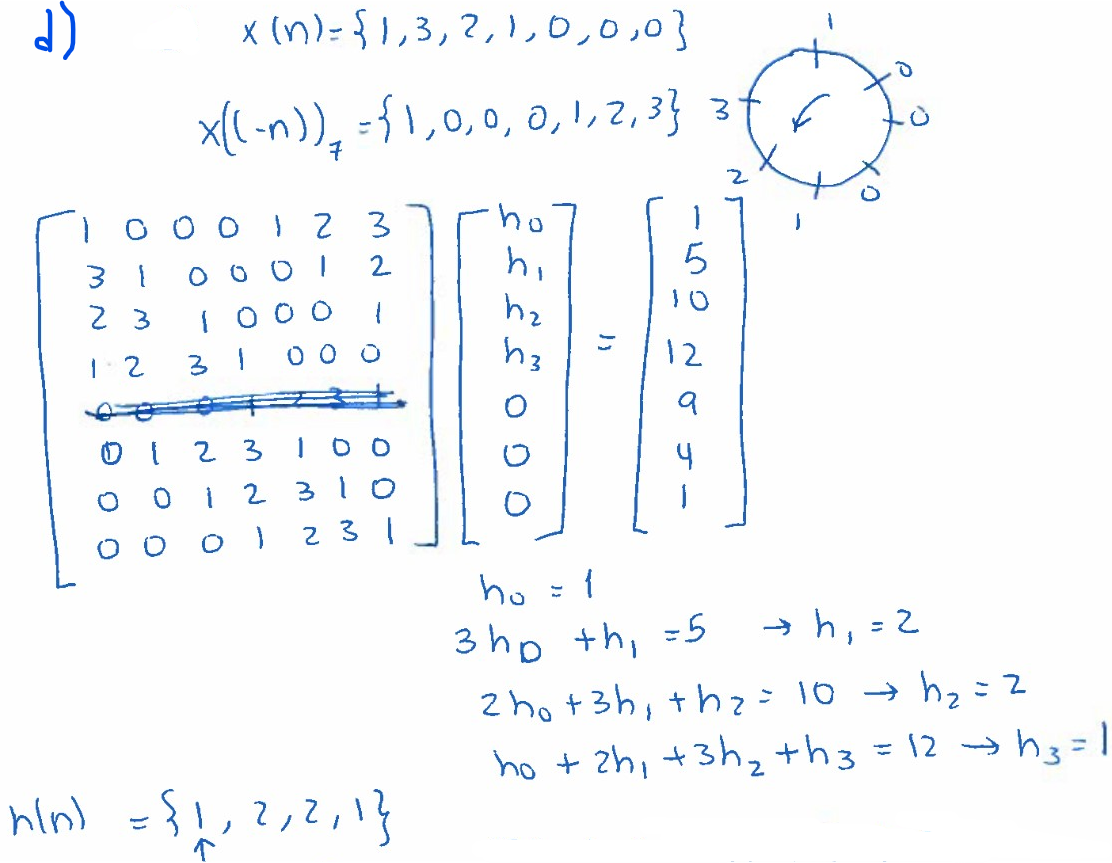
\includegraphics[width=.85\textwidth]{mt2_q2_d.png}
    \end{figure}
    \newpage
    \item {[35 points]} A digital filter is characterized by the following properties:
    \begin{itemize}
        \item The impulse response is real valued.
        \item It has two poles and two zeros.
        \item Peak of the frequency response occurs at $\frac{\pi}{2}$, and $\left|H\left(\frac{\pi}{2}\right)\right| = 1$.
        \item The poles are at a distance $r=0.8$ from the origin of the $z$-plane.
        \item One of the zeros is at the origin.
        \item Constant signals generate zero response from the system.
    \end{itemize}
    \begin{enumerate}
        \item {[4]} Sketch the pole-zero plot.
        \item {[8]} Find $H(z)$.
        \item {[5]} Write the difference equation describing the system.
        \item {[10]} Write down the expression for the magnitude response, $|H(\omega)|$, and sketch it roughly over $0\leq \omega \leq 1$. You do not have to give the perfect value for every $\omega$ but make sure that critical points are covered. What type of filter is this?
        \item {[8]} Determine the response of this system to the input $x[n]=3+\cos\left(\frac{\pi}{2}n+\frac{\pi}{4}\right).$
    \end{enumerate}
    \begin{figure}[H]
        \centering
        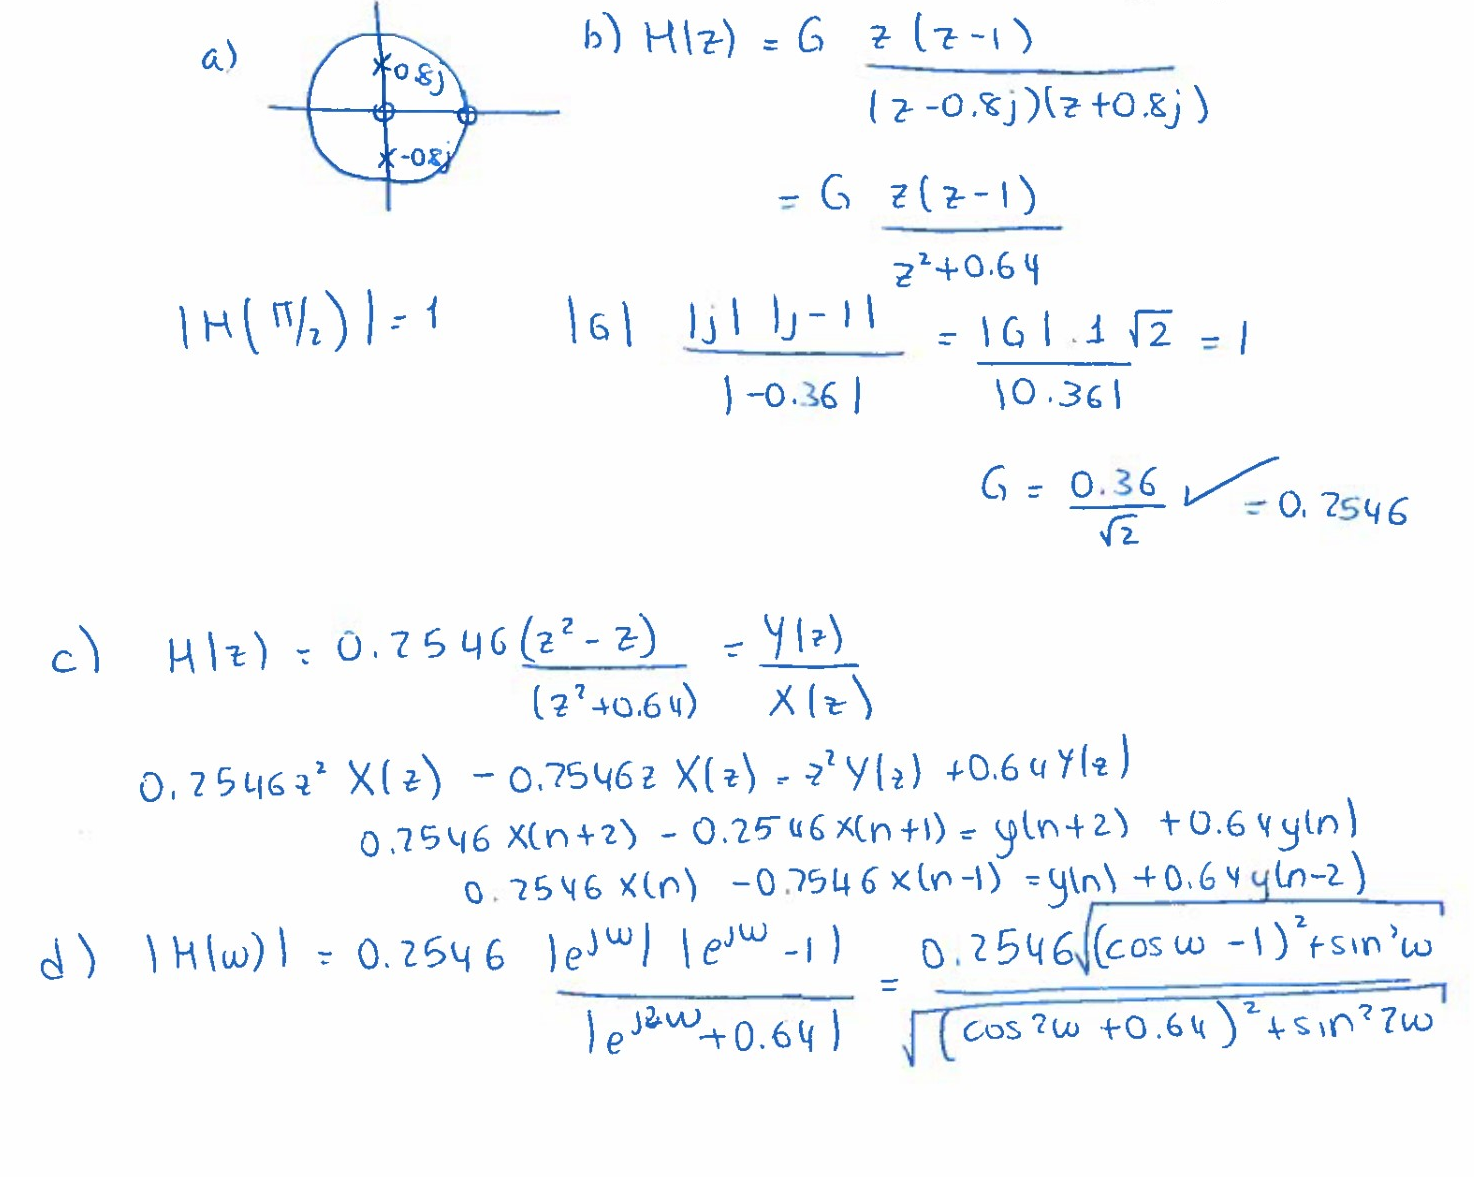
\includegraphics[width=\textwidth]{mt2_q3_a_d.png}
    \end{figure}

    \newpage
    \textit{Extra page for Question 3}
    \begin{figure}[H]
        \centering
        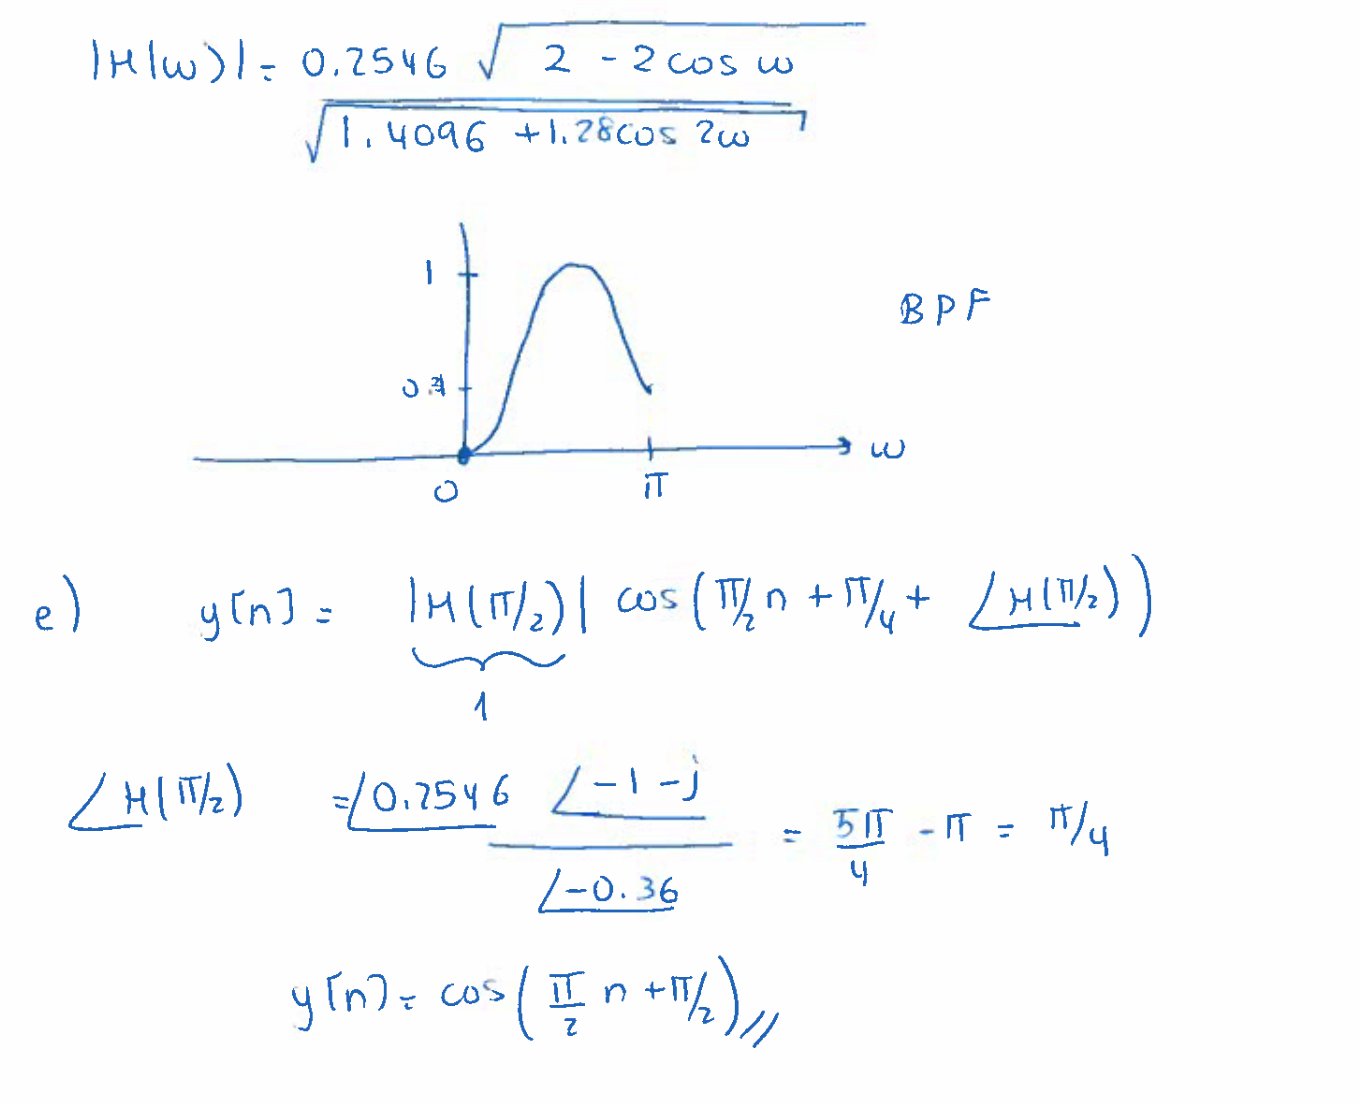
\includegraphics[width=\textwidth]{mt2_q3_d_e.png}
    \end{figure}
\end{enumerate}

\end{document}